\chapter{Result \& Evaluation}
% \addcontentsline{toc}{chapter}{Evaluation}
\label{ch:evaluation}

This chapter will provide the evaluation of the application via the experimental results and the overall visualization result. 

\section{Evaluation Method}

In order to evaluate the back-end machine learning approaches such as NER and deep learning models, accuracy, precision and F1 score can be used to examine the quality of the output result. Due to the human-readable characteristic of natural language, the feedback returned from the CV checker could be checked manually. Moreover, comparing with the result of existing systems and applications could also help to evaluate the performance of our application.


\section{Experimental Result}
Experimental results contain the results and evaluations for both dataset and all experimented back-end AI algorithms, including information extraction by NER, skill extraction and skill match.

\subsection{Information Extraction Result}
\label{sec:ner_result}

With the annotated resume dataset, which has been introduced in Section \ref{sec:data}, an NER model is trained for the information extraction task to check the CV content. The dataset is divided into the training set and test set with the ratio of 9:1. $Scorer.score$ module provided by spaCy is used to evaluate the NER model, which can calculate the precision, recall and f1 score of the model for each entity and the average score for all entities as well. The following table shows the evaluation result of our NER model, with the average score for all entities and the scores for some important entities. 


\begin{table}[htbp]
\centering
\begin{tabular}{|c|c|c|c|}
\hline
Entity Type & Precision & Recall & F1 Score\\
\hline
Name & 0.94 & 0.99 & 0.96\\
\hline
Designation & 0.58 & 0.72 & 0.65\\
\hline
Companies worked at & 0.72 & 0.77 & 0.74\\
\hline
Email Address & 0.94 & 0.95 & 0.95\\
\hline
Degree & 0.71 & 0.86 & 0.78\\
\hline
Skills & 0.50 & 0.35 & 0.41\\
\hline
Average & 0.63 & 0.57 & 0.60\\
\hline
\end{tabular}
\caption{Result of NER Model}
\label{tbl:4}
\end{table}

% too many types of entities, various of skill expressions, insufficient of training set

There are over fifteen types of named entities in the training set, some of which are not very common in resume data. In this case, the named entity labels in the training set are insufficient, and the obtained score of each entity are uneven. So, the average precision, recall and F1 score of all entities are not very high with about 0.60. By focusing on parts of results, the recognition results of the entities we are most concerned about are listed in the above Table \ref{tbl:4}. The obtaining scores for the basic information like Name and Email Address are pretty high with almost over 0.95, while the work experience recognition such as designation and companies are lower with around 0.70. As for the task of identifying skills in the resume, this NER model did not perform well though there are numerous annotations for skill entity. Through this result, it can be observed that recognition of the entities with similar patterns or expressions in different resumes such as Name and Email Address could get a high score. In contrast, the entities with diverse and complex expressions such as skills, obtained lower scores. Extending the training set could be one solution for getting a better result. According to \cite{fu2020interpretable}, the labeling consistency also affects the NER model, which could be regarded as the future work of our project.



\subsection{Data Analysis}

This section will give the visualization analysis of the job description dataset for skill extraction since visualization of the dataset can help the developer to have a deep understanding of the data for further processes. The job description dataset from Kaggle collected 19,001 job position details with 24 columns, including job title, company, job requirement, required qualification, etc. The column of job requirements is used in this project to obtain as many skills as possible.

After obtaining the tokens of the clean dataset by removing punctuation and special characters, the following figures show the word count and sentence count distribution of the job description (job requirement) text in the dataset, with a mean value of 95 words and eight sentences in each job description.

\begin{figure}[H]
    \begin{minipage}[t]{0.5\linewidth}
        \centering
        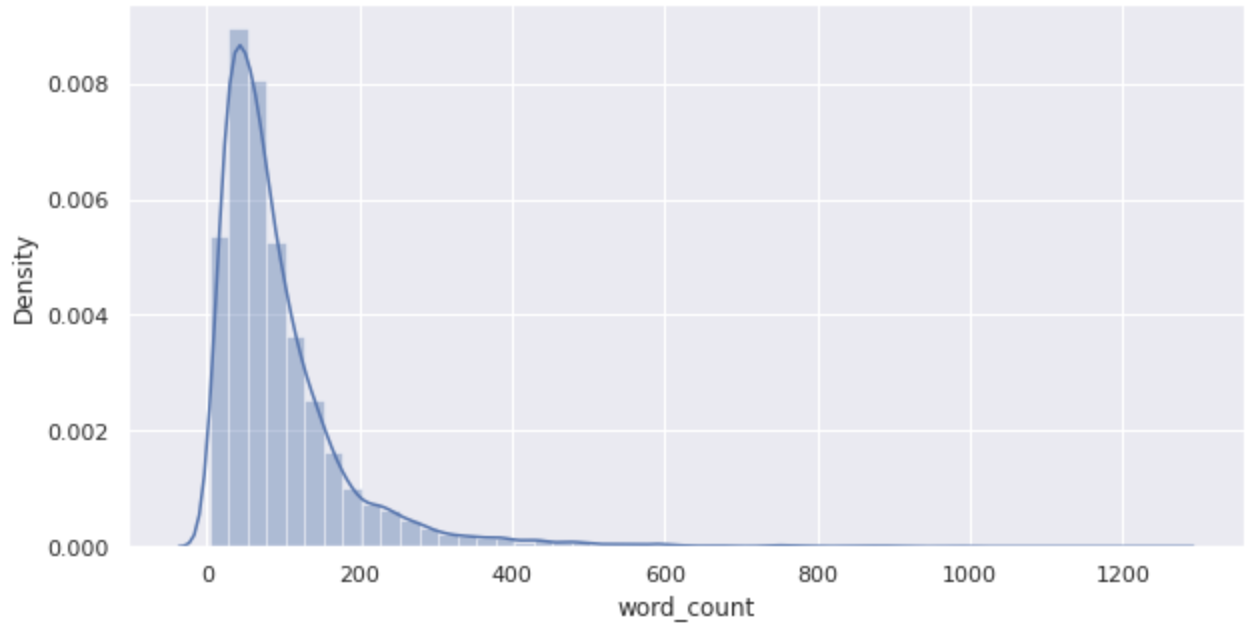
\includegraphics[scale=0.35]{images/wordcount.png}
        \caption{Word Distribution}
        \label{fig:21}
    \end{minipage}%
    \begin{minipage}[t]{0.5\linewidth}
        \centering
        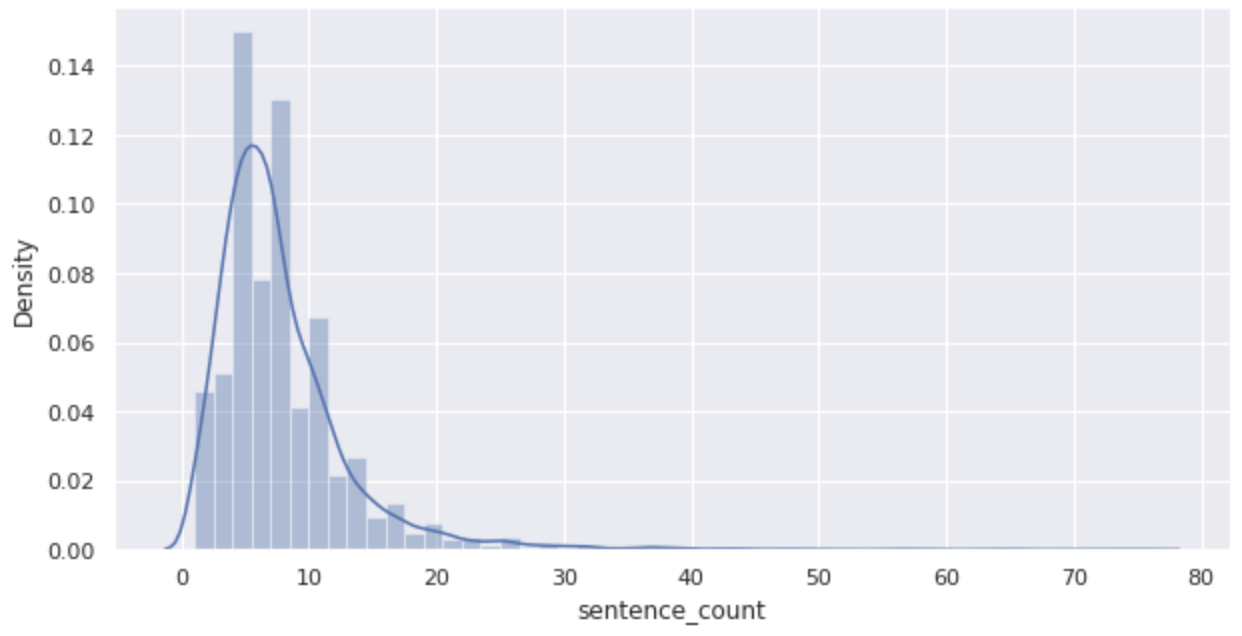
\includegraphics[scale=0.35]{images/sentencecount.png}
        \caption{Sentence Distribution}
        \label{fig:22}
    \end{minipage}
\end{figure}

With the preprocessing steps including stop words removal and lemmatization, the word frequency in the corpus is presented through histogram as Figure \ref{fig:23}. In order to see the words more straightforward, the most frequent words in the corpus are shown in Figure \ref{fig:24} via word cloud.

% \begin{figure}[H]
%     \centering
%     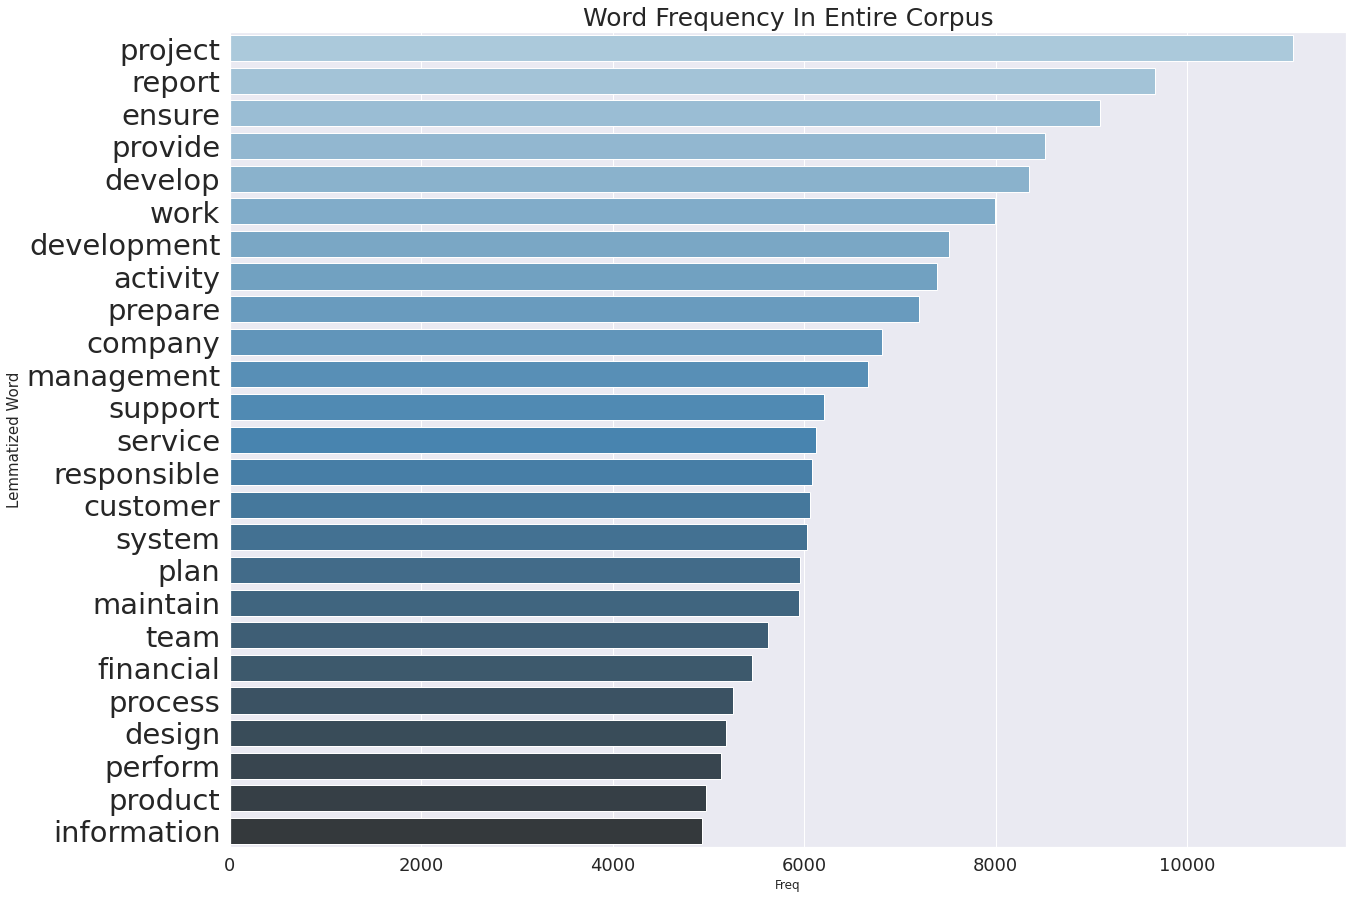
\includegraphics[width=0.7\textwidth]{images/frequent_hist.png}
%     \caption{Histogram of Word Frequency}
%     \label{fig:23}
% \end{figure}


% \begin{figure}[H]
%     \centering
%     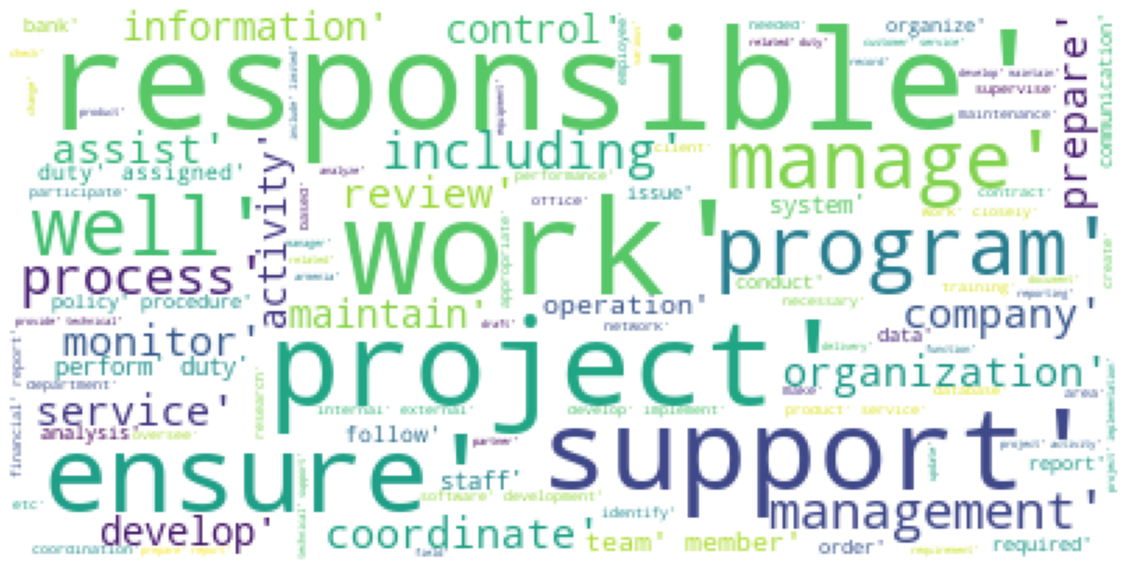
\includegraphics[width=0.6\textwidth]{images/frequent_cloud.png}
%     \caption{Word Cloud for Frequent Words}
%     \label{fig:24}
% \end{figure}

\begin{figure}[H]
    \begin{minipage}[t]{0.5\linewidth}
        \centering
        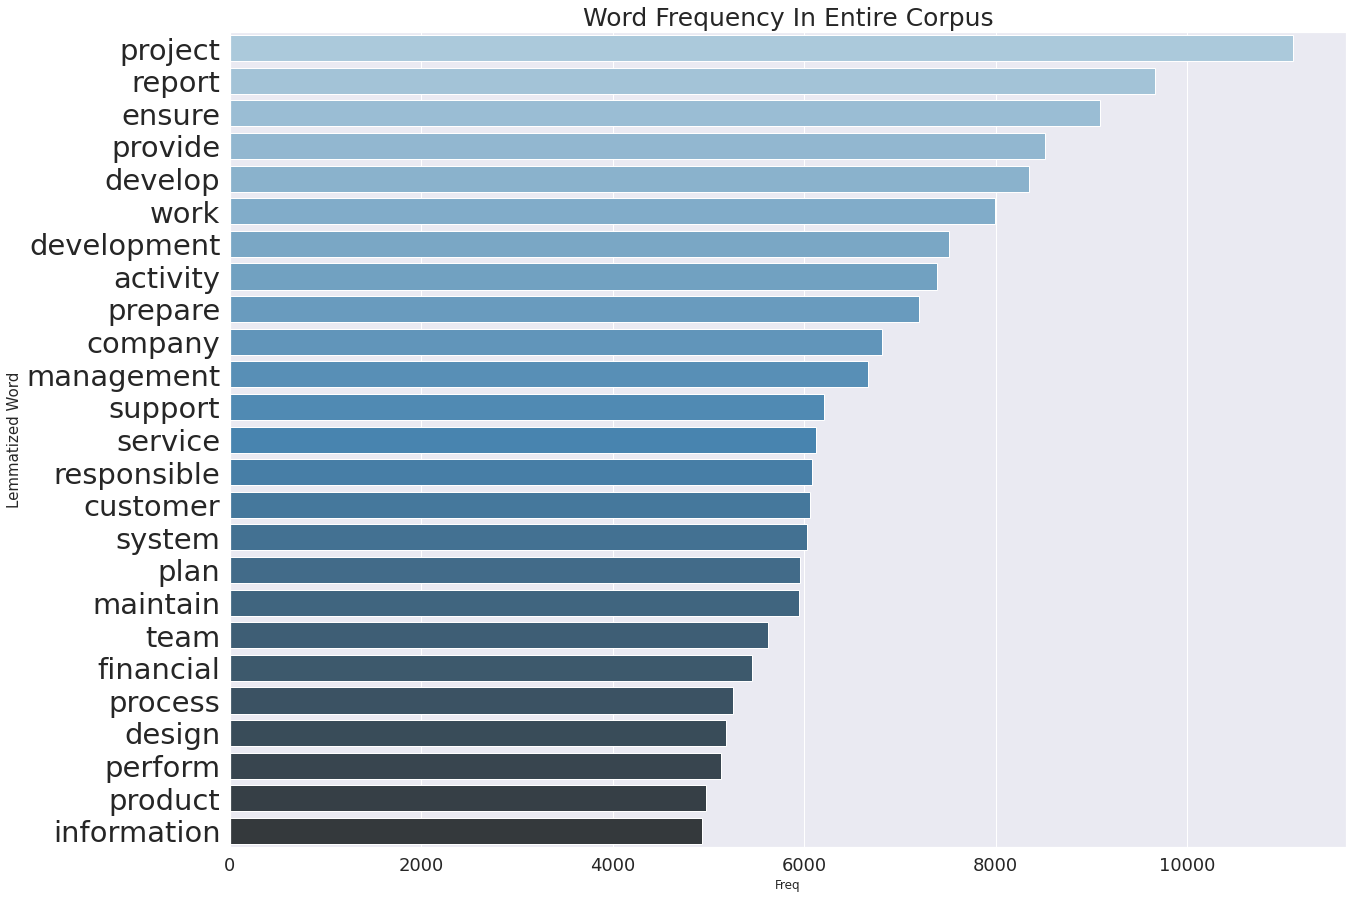
\includegraphics[scale=0.15]{images/frequent_hist.png}
        \caption{ Word Frequency Histogram}
        \label{fig:23}
    \end{minipage}%
    \begin{minipage}[t]{0.5\linewidth}
        \centering
        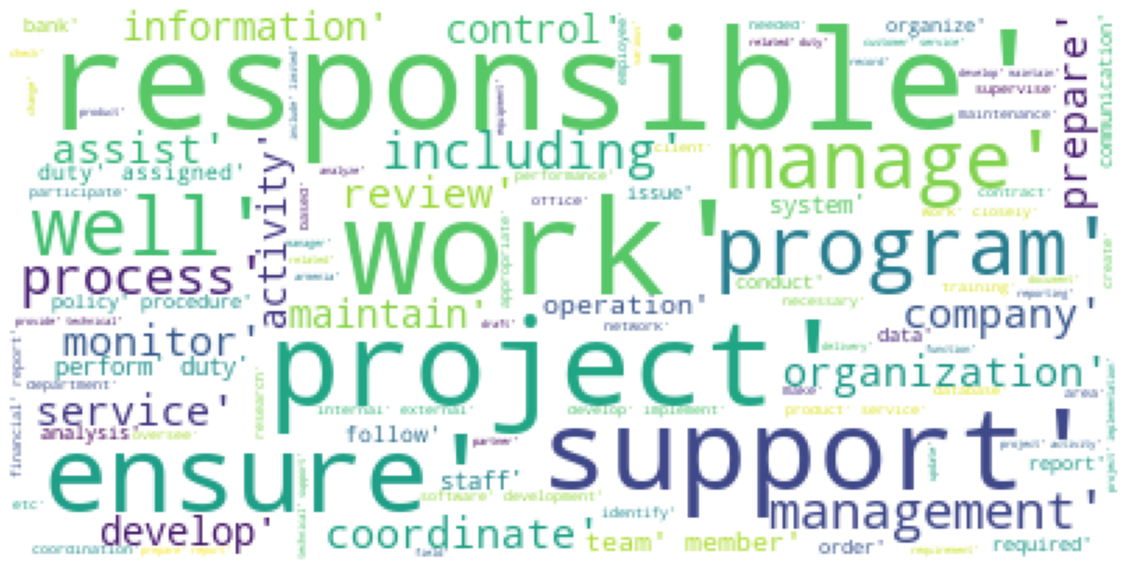
\includegraphics[scale=0.15]{images/frequent_cloud.png}
        \caption{Word Cloud}
        \label{fig:24}
    \end{minipage}
\end{figure}

According to the above figures, it seems that these top single words are indeed close to job positions but not totally skill-related. The most frequent n-grams (including Bigram and Trigram) are demonstrated as follows, which are more likely to be regarded as skill expressions than just single words. 

\begin{figure}[H]
    \begin{minipage}[t]{0.5\linewidth}
        \centering
        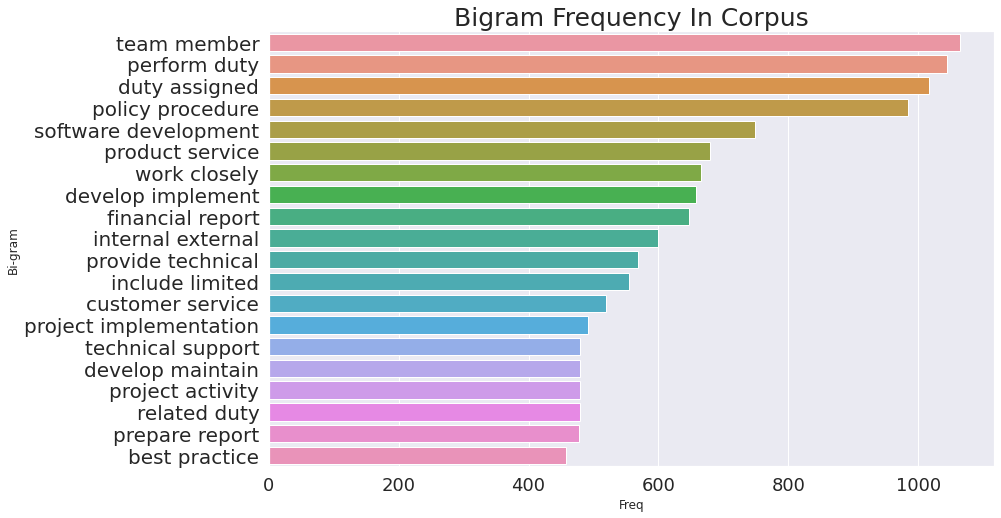
\includegraphics[scale=0.2]{images/bigram.png}
        \caption{Bigram Frequency}
        \label{fig:25}
    \end{minipage}%
    \begin{minipage}[t]{0.5\linewidth}
        \centering
        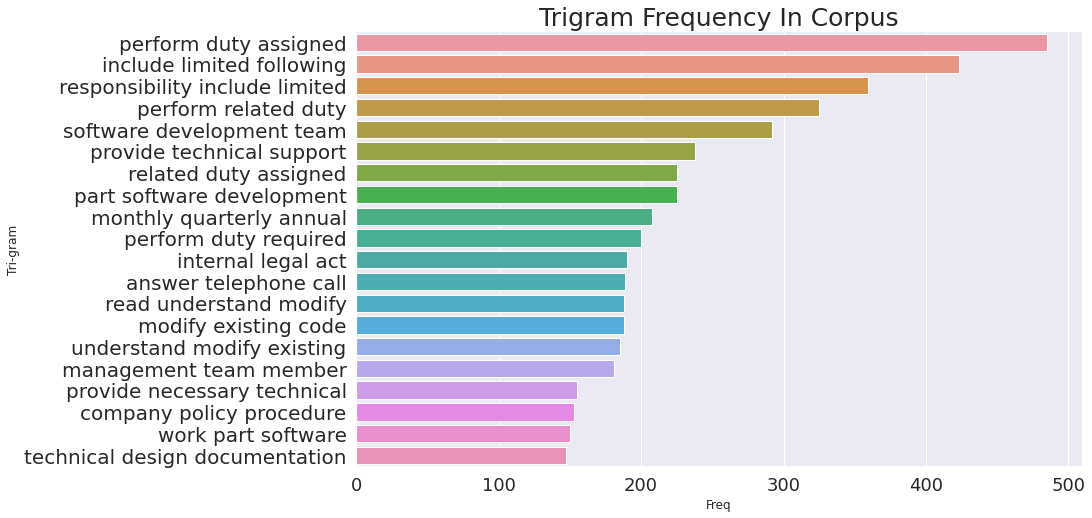
\includegraphics[scale=0.2]{images/trigram.png}
        \caption{Trigram Frequency}
        \label{fig:26}
    \end{minipage}
\end{figure}

% To gain the potential words and phrases for skills, POS tagging is used to get the chunks.


 \begin{figure}[H]
    \centering
    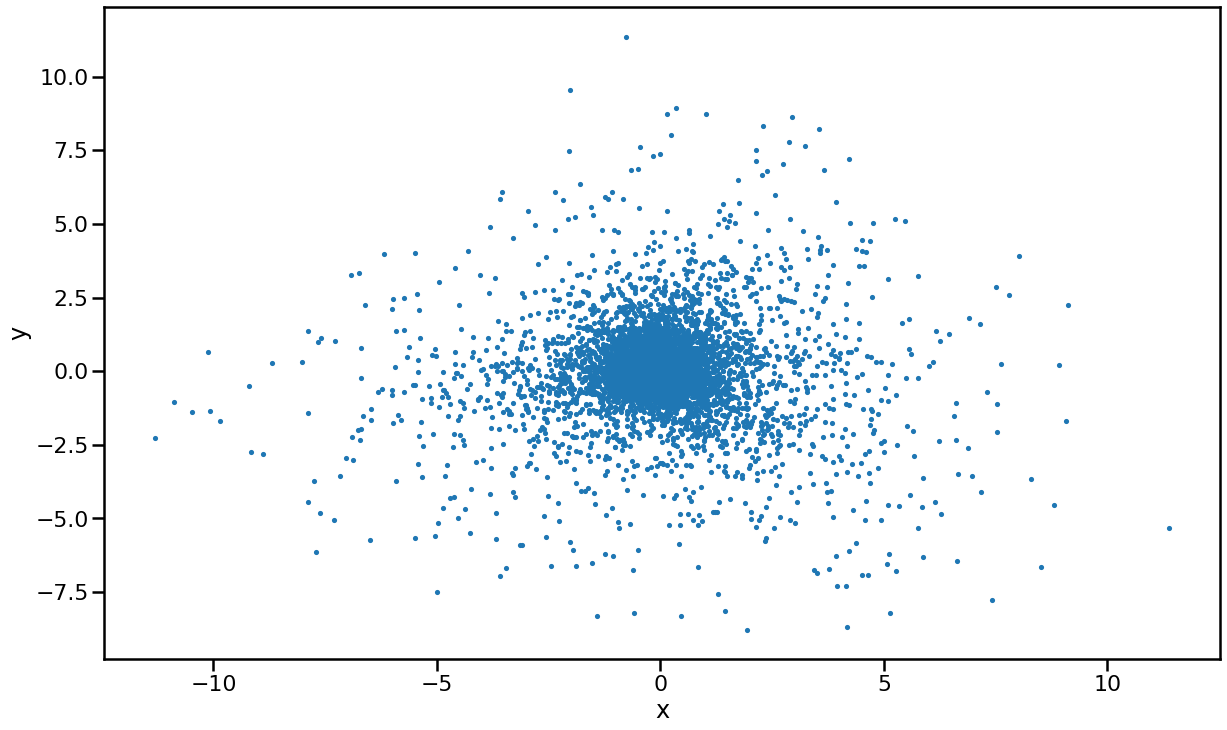
\includegraphics[width=1.0\textwidth]{images/word2vec_scatter.png}
    \caption{Scatter}
    \label{fig:27}
\end{figure}

\subsection{Skill Extraction Result}

\subsubsection{K-means Clustering}

The idea for using K-means algorithm to predict skills in the text is to get K clusters and expect some of the clusters to contain skills. As introduced in Section \ref{sec:word2vec}, word2vec is used to generate the word vectors for clustering. Based on Word2Vec model from Gensim and the pre-trained dataset  GoogleNews-vectors-negative300.bin.gz, which can be downloaded from \href{https://www.kaggle.com/datasets/leadbest/googlenewsvectorsnegative300}{kaggle}, we trained our word2vec model by the preprocessed job description dataset.

The dimension of the word vectors is set to 300; thus, to visualize the result of word2vec, Principle Components Analysis (PCA) is utilized to implement the dimensionality reduction from 300d to 2d. The scatter diagram of the word vectors is shown in Figure \ref{fig:27}, and a piece of the region of the vector points with the corresponding words is shown in Figure \ref{fig:28}.



\begin{figure}[H]
    \centering
    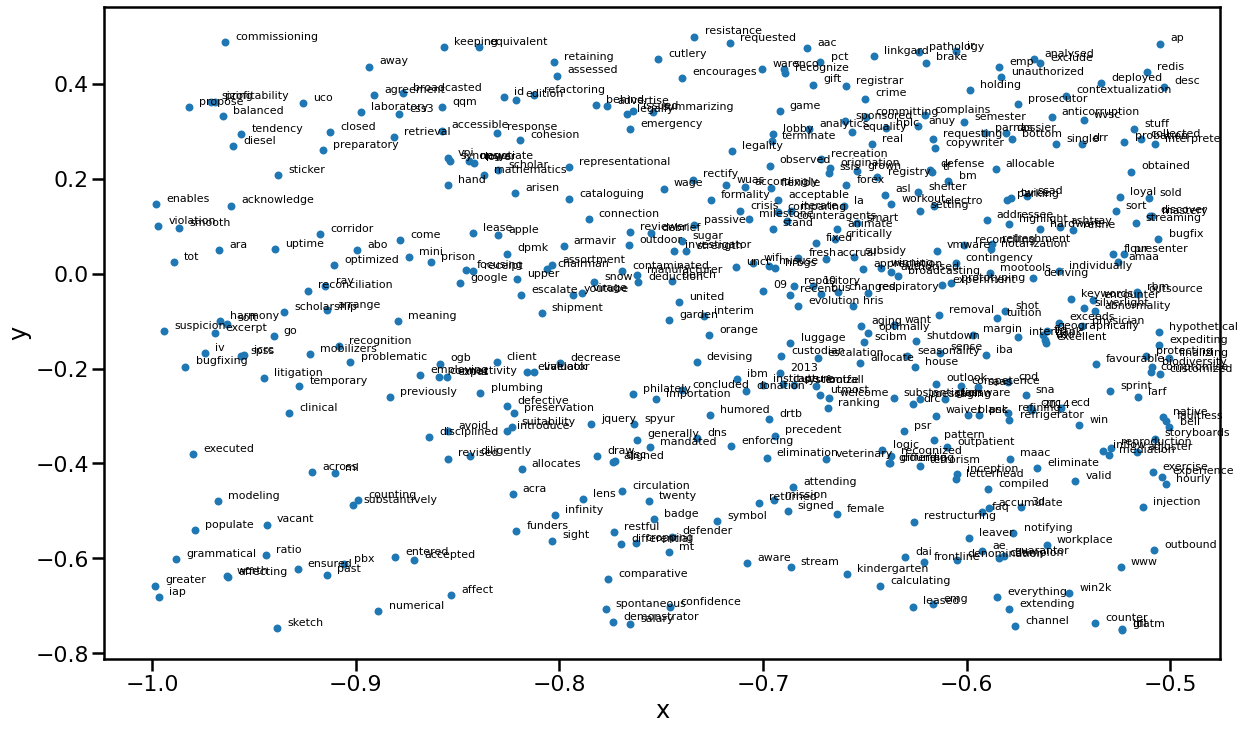
\includegraphics[width=1.0\textwidth]{images/word2vec_words.png}
    \caption{Scatter with Words}
    \label{fig:28}
\end{figure}

With the generated word vectors, the similarity between words can be calculated via 'similar\_by\_word' in Word2Vec module from Gensim. The following figures are screenshots demonstrating two examples, where the input word is the test word and the result presents the top 5 words most similar to the input word with their similarity. Through manual check, the related words computed by word vectors are reasonable, which means the word2vec model performs well.


\begin{figure}[H]
    \begin{minipage}[t]{0.5\linewidth}
        \centering
        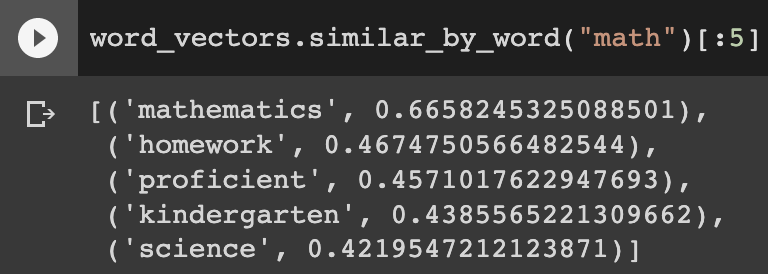
\includegraphics[scale=0.5]{images/wv_exp1.png}
        % \caption{Bigram Frequency}
        \label{fig:29}
    \end{minipage}%
    \begin{minipage}[t]{0.5\linewidth}
        \centering
        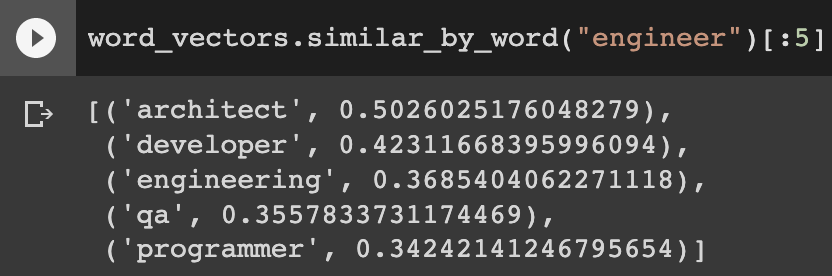
\includegraphics[scale=0.5]{images/wv_exp3.png}
        % \caption{Trigram Frequency}
        \label{fig:30}
    \end{minipage}
    \caption{Examples of Word Similarity}
\end{figure}

By using the word vectors as the training samples, K-menas algorithm could be applied to get clusters. Setting $n\_clusters$ to 12, top members, the 8 most close words of each clustering center, are listed in the following table \ref{tbl:2}. According to the result, some of the clusters are interpretable, where cluster $\#03$ is related to the information of bank or financial position, cluster $\#08$ might be about the verbs appeared in the job description and cluster $\#12$ could be connected to problem solving. But there is no cluster that obvious relate to skill as expected. The reason could be that the skill-related words are not all with the similar meanings, which means that the representation of those words would not be close to each other and would not be gathered in the same cluster. It is a common difficulty for clustering algorithm to deal with this kind of problem. The samples most close to the cluster center are regarded as the top words in K-means algorithm, but they are not the most representative and interpretable samples for the cluster in human-understanding. Moreover, K-means algorithm defines the members of the cluster based on Euclidean distance, and Euclidean distance could not work well in high dimensional data. Additionally, K-means can only detect spherical clusters, which might not fit this text dataset. Consequently, K-means clustering is not a suitable choice for the skill extraction task.


% \begin{figure}[H]
%     \centering
%     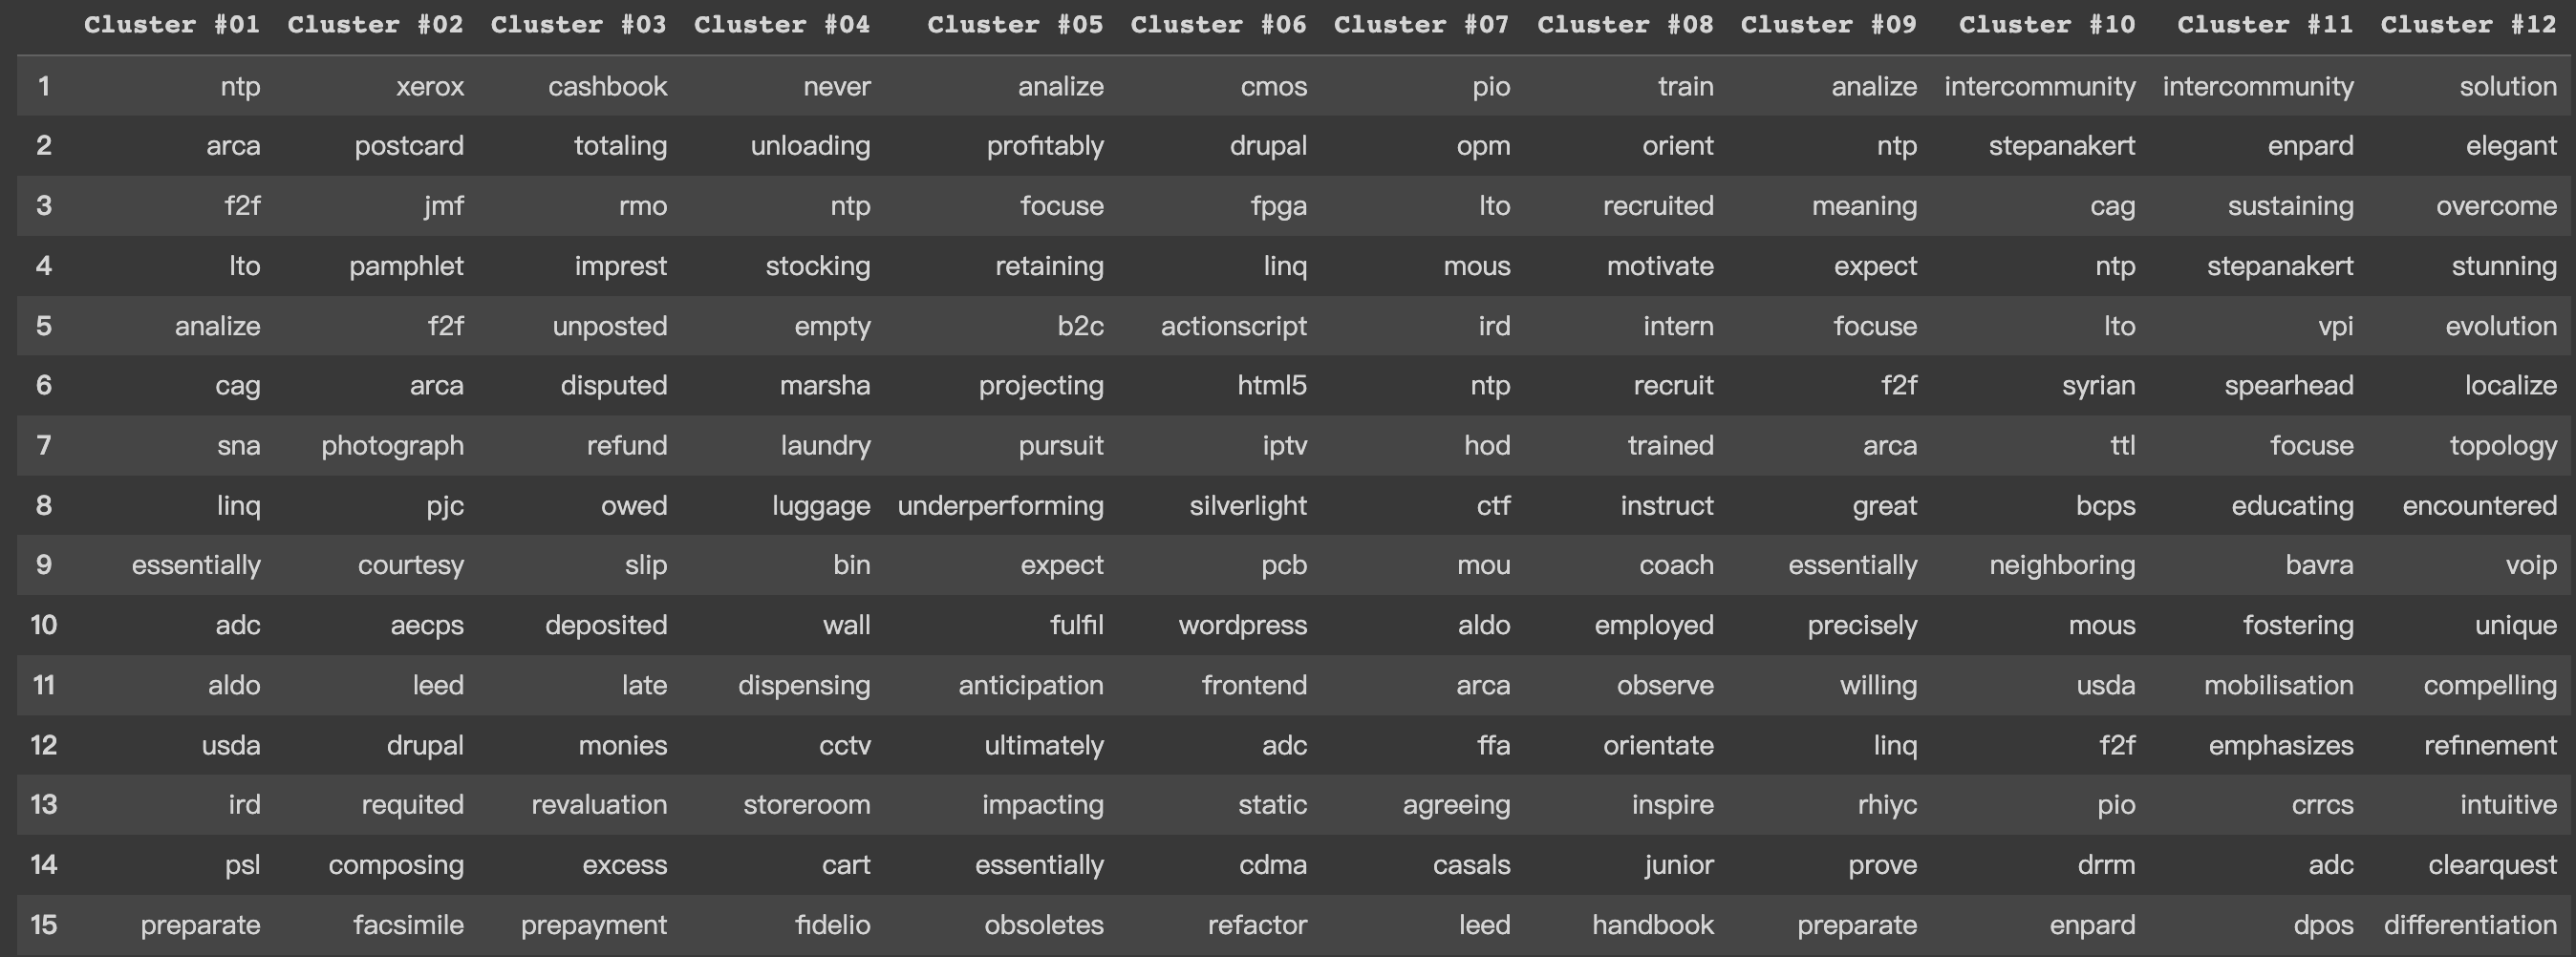
\includegraphics[width=1.0\textwidth]{images/kmeans_cluster.png}
%     \caption{K-means Clusters}
%     \label{fig:31}
% \end{figure}

\begin{table}[htbp]
\centering
\begin{tabular}{|c|c|}
\hline
Cluster ID & Top words\\
\hline
\#1 & ntp arca f2f lto analize cag sna linq\\
\hline
\#2 & xerox postcard jmf pamphlet f2f arca phtograph pjc\\
\hline
\#3 & cashbook totaling rmo imprest unposted disputed refund owed\\
\hline
\#4 & never unloading ntp stocking empty marsha laundry luggage\\
\hline
\#5 & analize profitably focuse retaining b2c projecting pursuit underperforming\\
\hline
\#6 & cmos drupal fpga linq actionscript html5 iptv silverlight\\
\hline
\#7 & plo opm lto mous ird ntp hod ctf\\
\hline
\#8 & train orient recruited motivate intern recruit trianed instruct \\
\hline
\#9 & analize ntp meaning expect focuse f2f arca great \\
\hline
\#10 & intercommunity stepanakert cag ntp lto syrian ttl bcps \\
\hline
\#11 & intercommunity enpard sustaining stepanakert vpi spearhead focuse educating \\
\hline
\#12 & solution elegant overcome stunning evolution localize topology encountered \\
\hline
\end{tabular}
\caption{K-menas Clusters}
\label{tbl:2}
\end{table}

\subsubsection{Topic Modeling}

Similar to the idea of K-means algorithm, topic modeling technique is also utilized to cluster the words in the corpus. The traditional topic model LDA models topics in each document and models words in each topic, which can make the cluster more meaningful and interpretable than K-means. A web application \href{https://palmetto.demos.dice-research.org}{Palmetto} is adopted to evaluate the coherence of obtained top words in each topic. With the input topic top words and a coherence measure selection, Palmetto service will calculate the different types of coherence and return the result. We chose $C_A$ to evaluate the topics, which computes the coherence based on word pairs, a context window, normalized pointwise mutual information (NPMI) and cosine similarity. The top words in each cluster generated by LDA with $topic\_number = 8$ and the coherence score are shown in the following Table \ref{tbl:3}. A few topics seem to be interpretable, and the top words from the LDA model represent the topic(cluster) more precisely than the central words from each centre of K-means model. Topic $\#2$ might be related to the descriptive words for market area and topic $\#5$ is like IT direction. However, the general coherence scores are low and still could not tell a cluster that points to skills. The result is not as expected since the unsupervised clustering algorithm generated the cluster most based on the meaning of the words instead of the category. Moreover, LDA can only model single words while many skill expressions appear as phrases. Therefore, LDA topic model is also not a good choice for this task, and the hybrid approach will be more appropriate.

\begin{table}[htbp]
\centering
\begin{tabular}{|c|c|c|}
\hline
Topic ID & Top words & $C_A$\\
\hline
\#1 & \tabincell{l}{responsible client report data \\develop new service test} & 0.17\\
\hline
\#2 & \tabincell{l}{product strategy manage market \\activity plan develop marketing} & 0.14 \\
\hline
\#3 & \tabincell{l}{information document make administrative \\perform duty provide staff} & 0.12\\
\hline
\#4 & \tabincell{l}{armenian material draft report \\project prepare assist provide} & 0.18\\
\hline
\#5 & \tabincell{l}{support employee database software \\procedure ensure equipment maintain} & 0.15 \\
\hline
\#6 & \tabincell{l}{plan staff training support development\\ implementation activity ensure} & 0.18\\
\hline
\#7 & \tabincell{l}{requirement develop application technical \\software project work development} & 0.28\\
\hline
\#8 & \tabincell{l}{procedure management credit ensure \\control accounting bank prepare} & 0.14\\
\hline
\end{tabular}
\caption{LDA Topics(Clusters)}
\label{tbl:3}
\end{table}


\subsubsection{Hybrid Approach}
\label{sec:bert}

Reviewing the details of the hybrid approach to extract skills in the job description, the main processes after preprocessing are: 1)POS tagging, 2) chunking by regular expressions to get potential skill expressions, 3)labeling the chunks to generate training data, 4)training Neural Network with BERT layer to binary classification.

Experimenting with chunking the data with the four regular expression patterns proposed by \cite{ketterer2}, the obtained chunks contain many unreasonable phrases such as meaningless nouns combination and long phrases with over five tokens, which are not as expected. We find out that in the originally proposed approach, they chunked the tokens directly without doing stop words removal and lemmatization for their dataset. In our implementation, the basic preprocessing steps were applied to our dataset to get a clearer result. Because of removing the stop words such as prepositions and pronouns, nouns and verbs were the main components of the dataset. In this case, the regular expression such as $\{<NN|NNS|NNP>+\}$ would not make sense anymore since there were many consecutive nouns in the dataset, but they should be separated into different chunks. Based on the observation during the experiment, the chunking rules are modified and the two patterns are used to extract the potential skill expressions, where we use constrained numbers to avoid long meaningless noun phrases:

\begin{enumerate}
    \item Noun Phrase: $\{<JJ>*<NN|NNS|NNP>\{1,3\}\}$
    
    \item Verb Phrase: $\{<VBG|VBZ|VBP|VBD|VB|VBN><JJ>*<NNS|NN>\{0,3\}\}$
\end{enumerate}

Over 50,000 chunks are generated in two pickle files with a ratio of 7:3 (Noun Phrase to Verb Phrase) by utilizing the above two regular expression patterns. Since the phrases need to be labeled manually, the sample size should be reduced as much as possible. In order to ensure the samples can represent the characteristics of the original data, the appropriate number of samples is drawn out from each pickle file based on the size ratio of the files. $DataFrame.sample()$ is applied to sample the data randomly. Eventually, around 2,500 phrases are sampled from the pickle files and combined with a text file which contains over 1,500 skills to enrich the training set. The final training data contains over 4,000 phrases, and after labeling, the balance of the training set is shown as the following Figure \ref{fig:32}. 

 \begin{figure}[H]
    \centering
    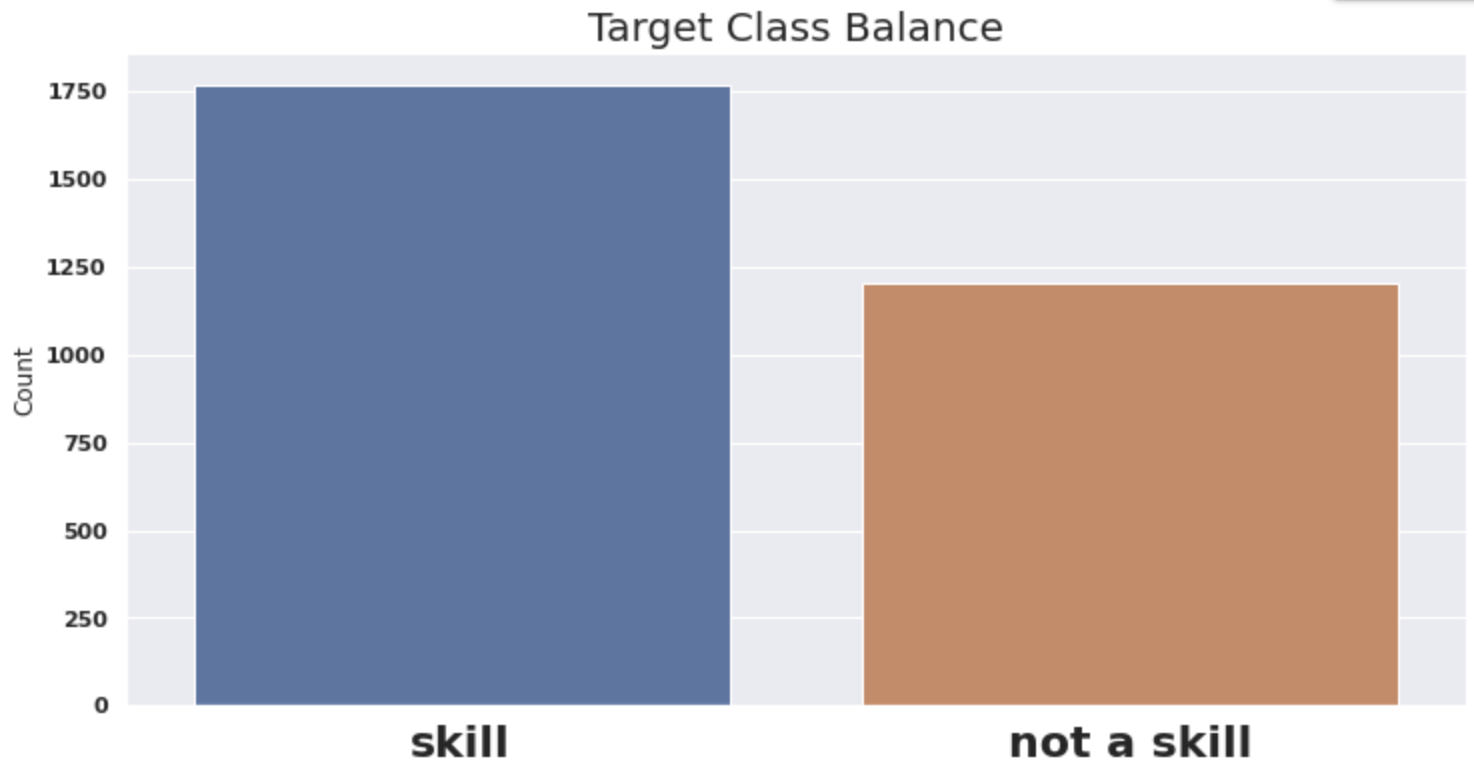
\includegraphics[width=0.8\textwidth]{images/training_set_balance.png}
    \caption{Training Set}
    \label{fig:32}
\end{figure}

Completing building the training dataset, the deep learning neural network with BERT layer is trained to classify the phrases to skill or not skill. The model is built based on Keras in Tensorflow, and the description of layers in the network is as follows:

 \begin{figure}[H]
    \centering
    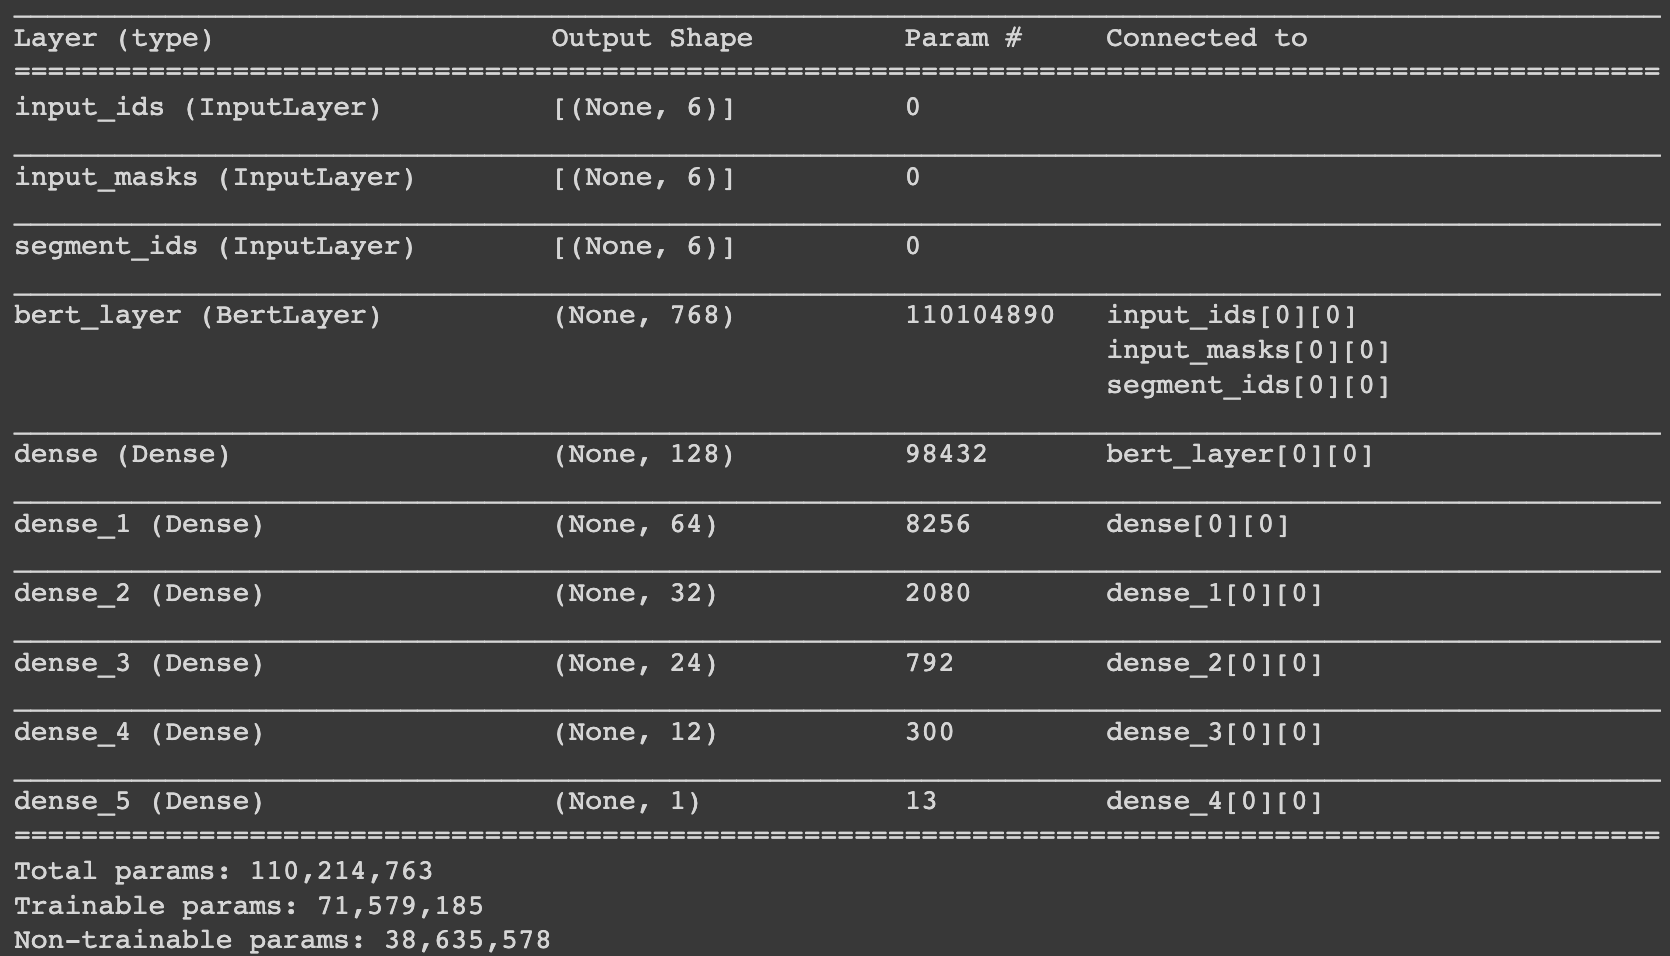
\includegraphics[width=1.0\textwidth]{images/layers_bert.png}
    \caption{Layers of the Classification Model}
    \label{fig:33}
\end{figure}

Splitting the dataset into training and validation data by the proportion of 0.8, the total loss and the accuracy results for both the training set and validation set during training in each epoch are demonstrated in the following figures.

\begin{figure}[H]
    \begin{minipage}[t]{0.5\linewidth}
        \centering
        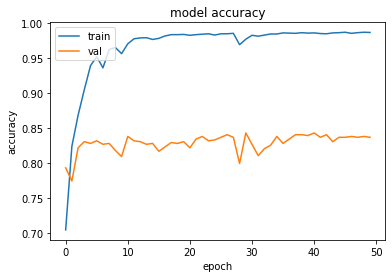
\includegraphics[scale=0.5]{images/acc_graph.png}
        % \caption{Bigram Frequency}
    \end{minipage}%
    \begin{minipage}[t]{0.5\linewidth}
        \centering
        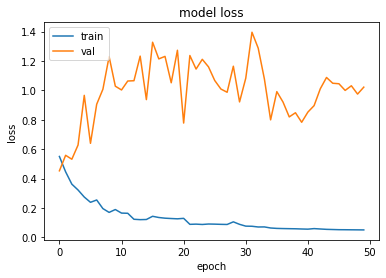
\includegraphics[scale=0.5]{images/loss_graph.png}
        % \caption{Trigram Frequency}
    \end{minipage}
    \label{fig:34}
    \caption{Accuracy \& Loss of the Classification Model}
\end{figure}


% \begin{table}[htbp]
% \centering
% \begin{tabular}{|c|c|c|c|c|}
% \hline
% Epoch & Train\_acc & Val\_acc & Train\_loss & Val\_loss\\
% \hline
% 5 & 0.95 & 0.83 & 0.16 & 0.62\\
% \hline
% 10 & 0.97 & 0.83 & 0.14 & 1.23\\
% \hline
% 15 & 0.98 & 0.83 & 0.04 & 0.91\\
% \hline
% 20 & 0.98 & 0.84 & 0.06 & 0.89\\
% \hline
% 30 & 0.99 & 0.82 & 0.05 & 1.11\\
% \hline
% \end{tabular}
% \caption{Result of Classification Model}
% \label{tbl:5}
% \end{table}

According to Figure \ref{fig:34}, the loss of validation data during 50 epochs is unstable and has a trend towards increasing, though the accuracy and loss of the training set continuously decline, which means the model might encounter the overfitting problem. To balance the total loss and the accuracy of both the train and validation data, the number of epochs is set to 20. Then, the BERT model got an accuracy of 0.98 with the training data, and 0.84 with the validation data.

In addition, another piece of job posting text from the Internet was tested as unseen data. After preprocessing and chunking the text, the extracted phrases from the data are manually labeled to get the prediction result. Dealing with this unseen data, our model got an accuracy of 0.75 and a loss of 3.88. The accuracy of the model on the testing data is acceptable. However, some phrases are not very interpretable, which will be discussed in Section \ref{sec:visual} with the visualization result. 




\subsection{Matching Result}

The original idea of matching the resume to the position is to match their skills on the condition that most skills are extracted. But as mentioned in Section \ref{sec:ner_result}, the performance of the NER model on recognizing skills in the resume was not as expected. Several real-world resumes were tested but few skills were extracted successfully. Therefore, we decided to use cosine similarity between the whole resume text and the job description to get the final match rate. The result is hard to be quantitatively evaluated since there is no standard measure to determine the match rate of two text data. So we compared our result with an existing robust CV checker \href{https://careerset.com/}{CareerSet} via different test cases to check whether our result is reasonable. The following table shows the match rate results from CareerSet and our application.

\begin{table}[htbp]
\centering
\begin{tabular}{|c|c|c|c|}
\hline
Test Case & CareerSet & Our Application\\
\hline
1 & 43\% & 50.42\%\\
\hline
2 & 75\% & 48.34\%\\
\hline
3 & 47\% & 62.1\% \\
\hline
\end{tabular}
\caption{Comparison of Match Rate Result}
\label{tbl:5}
\end{table}

The three test cases used the same resume and targeted to three different kinds of positions. According to the result, for low matching, such as test case 1, the result of our application is close to that from CareerSet. For case 2, the resume and the target position should have a high match, while our application generated a low match result. It is a limitation of regarding the cosine similarity of entire contents as the match rate between the resume and the target position. Because resume and job description data have totally different styles, the high match rate does not need the high similarity of the contents. 


\section{Overall Evaluation}
\label{sec:visual}



Based on the techniques for content checking and skill extraction, the visualization result of the application is shown in the following Figure \ref{fig:36}. The match rate from the resume to the job description is presented at the top of the page. As for the resume content check, according to the figure, the checklist contains Name, Email address, College, Degree, Designation and Skills. When recognizing the entities in the resume, the content of the named entity will be shown in the table. If the entity on the checklist has not been detected, the content column will print 'Not Detected' instead. The input resume contains all named entities on the checklist, but the email address and skills are not detected by our application, which is caused by the performance of the NER model. 

The extracted skills from the job description are listed at the bottom of the page. As illustrated in Section \ref{sec:bert}, though the deep learning model with BERT layer got high accuracy, the chunks predicted to be skills are not entirely reasonable and interpretable. According to the extracted skills listed in the figure, some irrelevant nouns were chunked together based on the regex patterns, and some chunks contained more than one skill. Setting more different regex for chunking might get a better result, but since the representation of skills is various, it is hard to define the most suitable regex chunking patterns. It can be regarded as the limitation of the regex-based chunking algorithm to extract phrases. Moreover, some phrases were not skill-related but were classified as skill, while some skills were predicted to be non-skill, which might be caused by the performance of the BERT model. The neural network training set needs to contain more job position fields to cover more skills in different areas. Furthermore, since the training data was labeled manually, labeling mistakes could not be eliminated, which would also affect the prediction result.


% 1. (limitation) chunks might got wrong, combinition of several skills
% 2. training set does not contain enough field of job
% 3. more or different regex might be found for better result
% 4. BERT NN part is fine
% 5. manual labeling with mistakes

 \begin{figure}[H]
    \centering
    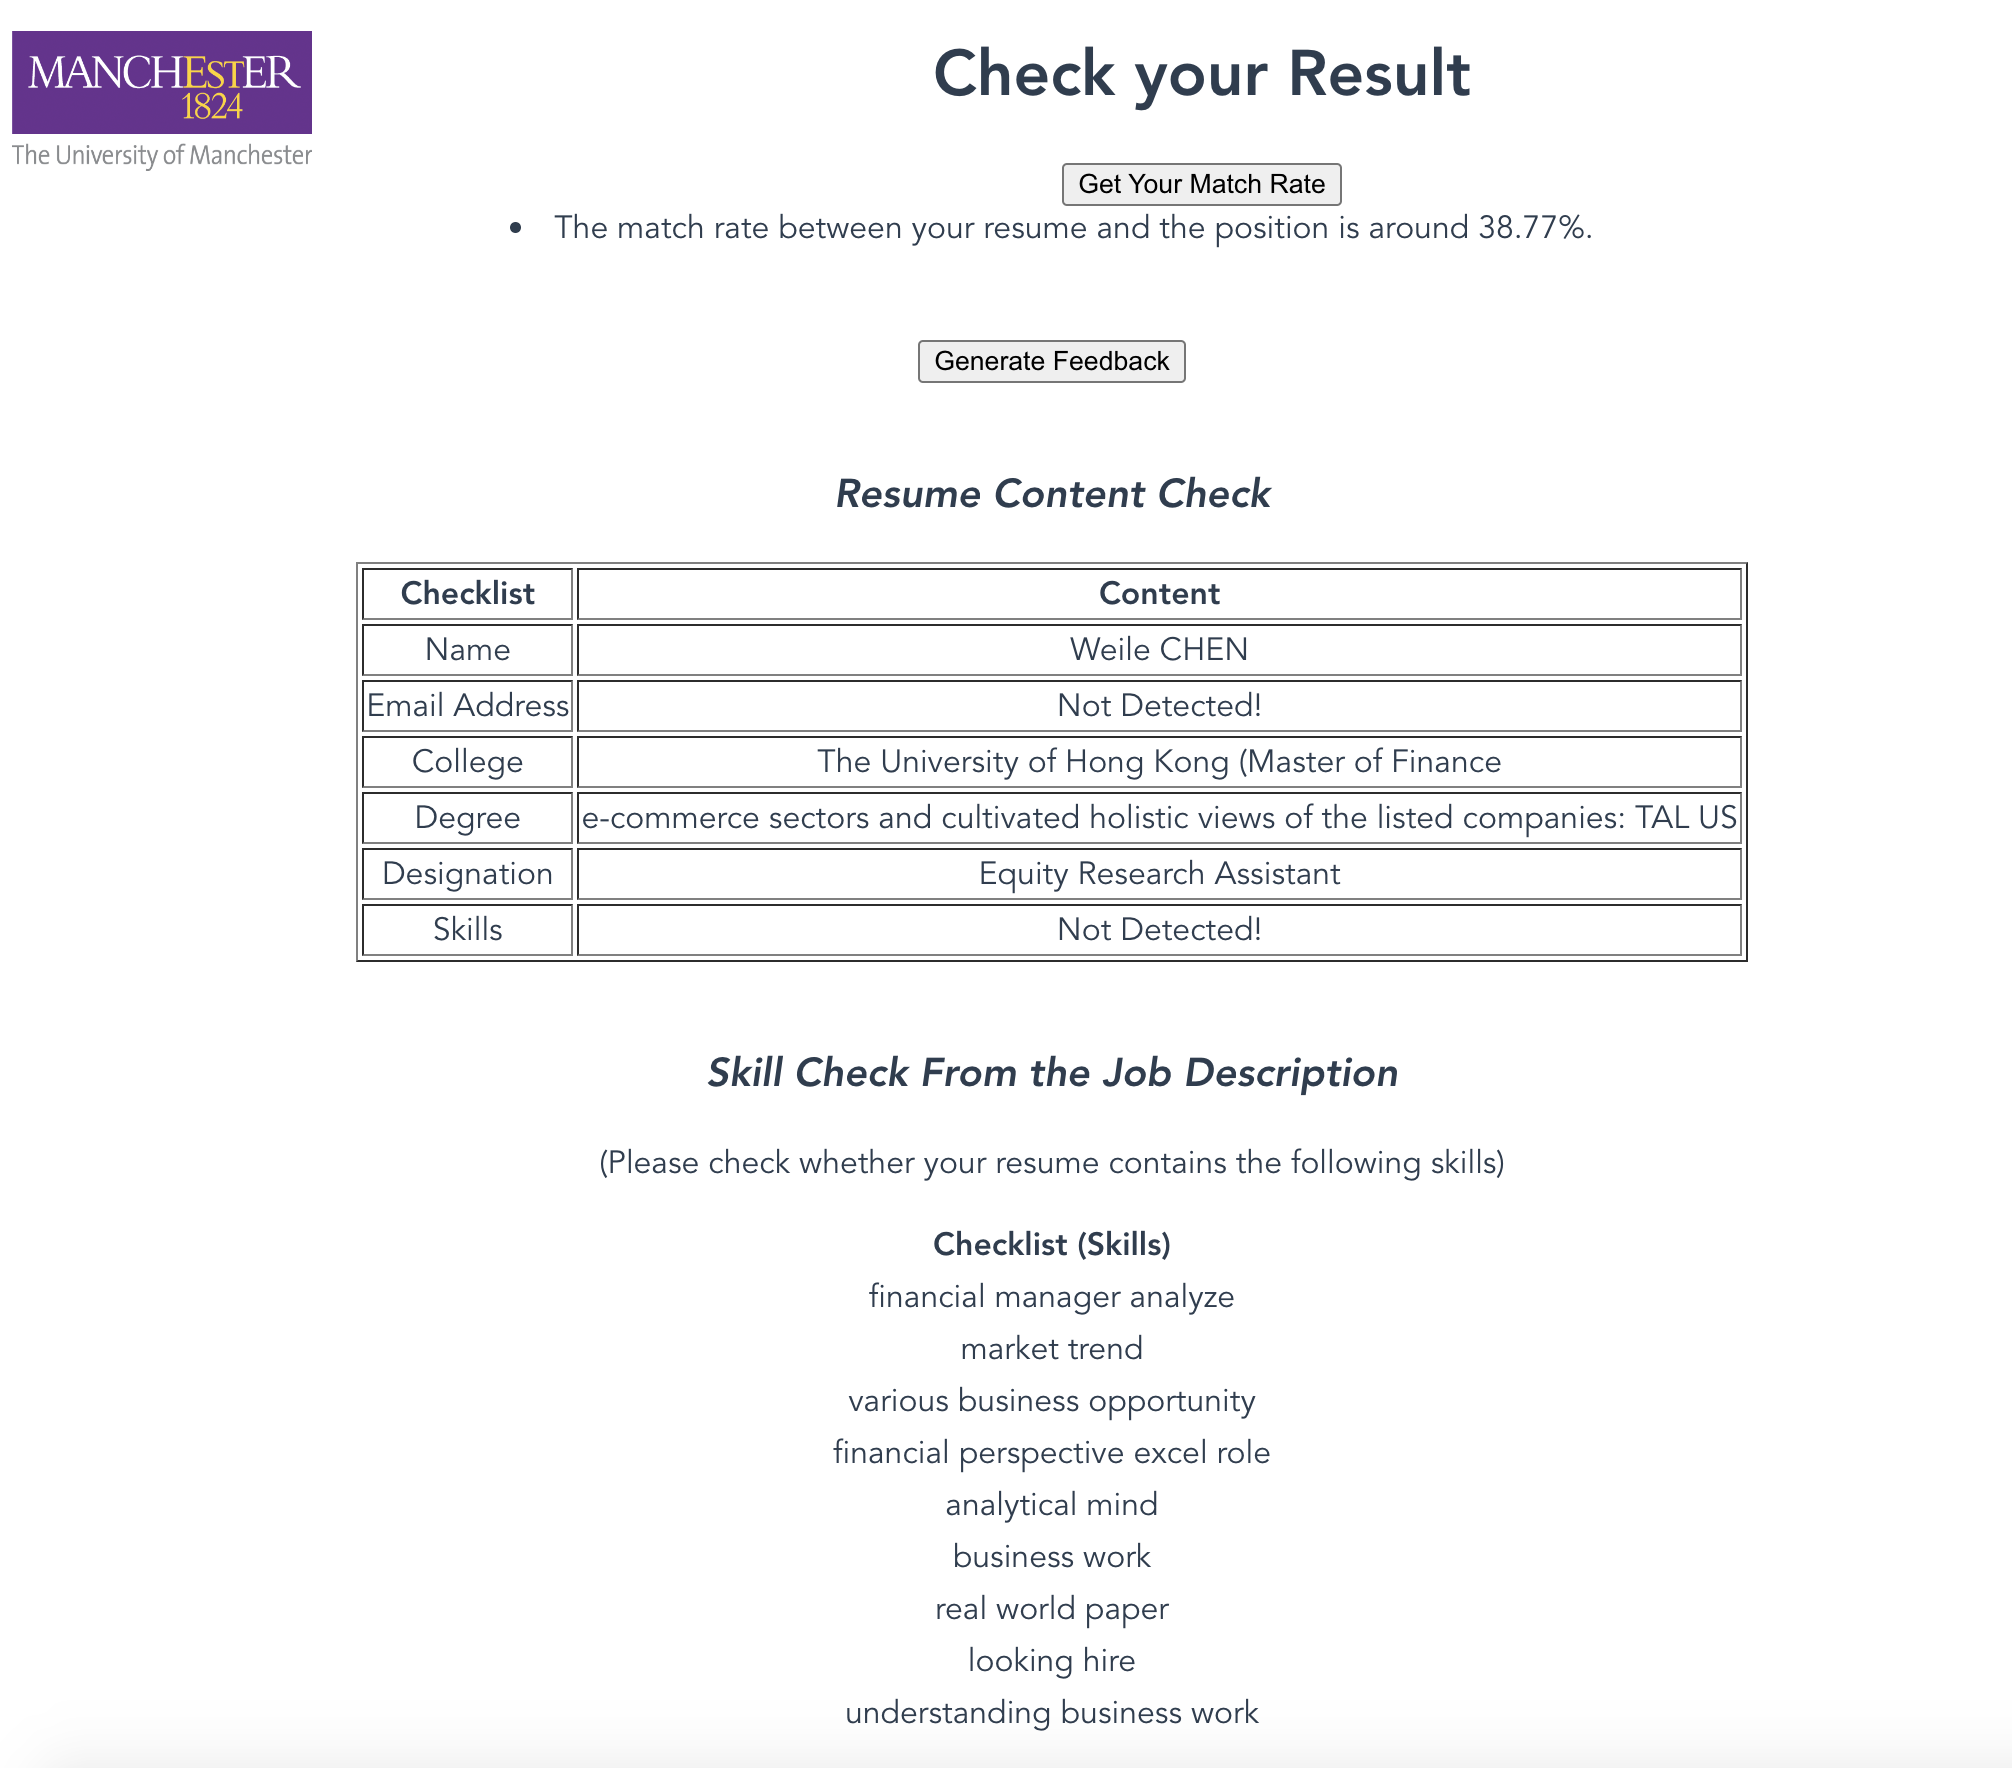
\includegraphics[width=1.1\textwidth]{images/visual.png}
    \caption{Screenshot of the Feedback Page}
    \label{fig:36}
\end{figure}
